\documentclass[10pt,leqno]{article}

\usepackage[%
  tmargin=1.2in,bmargin=1.2in,%
  lmargin=1.8in,rmargin=1.8in,%
]{geometry}
\usepackage{fancyhdr}
\usepackage{titlesec}
\usepackage{appendix}
\usepackage{microtype}
\usepackage[hyphens]{url}
\usepackage{enumitem}
\usepackage{xspace}
\usepackage{etoolbox}
\usepackage{ifthen}
\usepackage{tikz}
\usepackage{tikz-cd}

\usepackage{amsmath}
\definecolor{darkred}{rgb}{0.5,0.0,0.0}
\usepackage[%
  colorlinks,%
  linkcolor=darkred,%
  citecolor=darkred,%
  urlcolor=darkred,%
]{hyperref}
\usepackage{amsthm,amssymb}
% \usepackage[lining,semibold]{libertine}
% \usepackage{textcomp,stmaryrd}
% \usepackage[libertine,cmintegrals,bigdelims]{newtxmath}
% \useosf
% \usepackage[%
%   cal=boondox, calscaled=0.97,%
%   bb=boondox, bbscaled=0.98,%
% ]{mathalfa}
\usepackage{cleveref}

\frenchspacing
\urlstyle{rm}

\AtBeginDocument{%
  \setlength{\abovedisplayskip}{1.5ex plus 0.3ex minus 0.3ex}%
  \setlength{\abovedisplayshortskip}{1.0ex plus 0.3ex minus 0.3ex}%
  \setlength{\belowdisplayskip}{1.5ex plus 0.3ex minus 0.3ex}%
  \setlength{\belowdisplayshortskip}{1.0ex plus 0.3ex minus 0.3ex}%
}

\let\theoldbibliography\thebibliography
\renewcommand{\thebibliography}[1]{%
  \theoldbibliography{#1}%
  \setlength{\parskip}{0ex}
  \setlength{\itemsep}{0.5ex plus 0.2ex minus 0.2ex}
  \small
}

\pagestyle{fancy}
\renewcommand{\headrulewidth}{0pt}
\renewcommand{\footrulewidth}{0pt}
\fancyhf{}
\fancyfoot[C]{\small\thepage}

\renewcommand{\title}[1]{\newcommand{\thetitle}{#1}}
\renewcommand{\author}[1]{\newcommand{\theauthor}{#1}}
\renewcommand{\date}[1]{\newcommand{\thedate}{#1}}

\renewcommand{\maketitle}{%
  \begin{center}
    {\bfseries\MakeUppercase{%
      \thetitle}}\\[2.5ex]
    {\footnotesize\MakeUppercase{%
      \theauthor}}\\[2.5ex]
    \ifthenelse{\equal{\thedate}{}}{}{%
      \small%
      \setlength{\tabcolsep}{0.2em}%
      \begin{tabular}{rl}
        original: & \thedate \\
        updated: & \today
      \end{tabular}
    }
  \end{center}
  \vspace{2.5ex}
  \thispagestyle{fancy}
}

%%%%%%%%%%%%%%%%%%%%%%%%%%%%%%%%%%%%%%%%%%%%%%%%%%%%%%%%%%%%%%%%%%%%%%

\cspreto{section}{\setcounter{equation}{0}}

\titleformat{\section}{\centering\scshape}{\thesection.}{0.4em}{}
\titlespacing{\section}{0pt}{*4}{*1}
\titleformat{\subsection}{\scshape}{\thesubsection.}{0.4em}{}
\titlespacing{\subsection}{0pt}{*2.5}{*1}

% Display format for equations
\newcommand{\crefeqfmt}[1]{
  \crefformat{#1}{(##2##1##3)}
  \Crefformat{#1}{(##2##1##3)}
  \crefrangeformat{#1}{(##3##1##4--##5##2##6)}
  \Crefrangeformat{#1}{(##3##1##4--##5##2##6)}
  \crefmultiformat{#1}{(##2##1##3}{, ##2##1##3)}{, ##2##1##3}{, ##2##1##3)}
  \Crefmultiformat{#1}{(##2##1##3}{, ##2##1##3)}{, ##2##1##3}{, ##2##1##3)}
  \crefrangemultiformat{#1}{(##3##1##4--##5##2##6}{, ##3##1##4--##5##2##6)}{, ##3##1##4--##5##2##6}{, ##3##1##4--##5##2##6)}
  \Crefrangemultiformat{#1}{(##3##1##4--##5##2##6}{, ##3##1##4--##5##2##6)}{, ##3##1##4--##5##2##6}{, ##3##1##4--##5##2##6)}
}
% Display format for sections
\newcommand{\crefsecfmt}[1]{%
  \crefformat{#1}{\S##2##1##3}
  \Crefformat{#1}{\S##2##1##3}
  \crefrangeformat{#1}{\S\S##3##1##4--##5##2##6}
  \Crefrangeformat{#1}{\S\S##3##1##4--##5##2##6}
  \crefmultiformat{#1}{\S\S##2##1##3}{ and~##2##1##3}{, ##2##1##3}{ and~##2##1##3}
  \Crefmultiformat{#1}{\S\S##2##1##3}{ and~##2##1##3}{, ##2##1##3}{ and~##2##1##3}
  \crefrangemultiformat{#1}{\S\S##3##1##4--##5##2##6}{ and~##3##1##4--##5##2##6}{, ##3##1##4--##5##2##6}{ and~##3##1##4--##5##2##6}
  \Crefrangemultiformat{#1}{\S\S##3##1##4--##5##2##6}{ and~##3##1##4--##5##2##6}{, ##3##1##4--##5##2##6}{ and~##3##1##4--##5##2##6}
}
\crefeqfmt{equation}
\crefeqfmt{enumi}
\crefeqfmt{enumii}
\crefsecfmt{section}
\crefsecfmt{subsection}
\crefsecfmt{appendix}
\crefname{part}{Part}{Parts}
\crefname{chapter}{Chapter}{Chapters}
\crefname{figure}{Figure}{Figures}

\makeatletter

\newcommand{\thmnumfont}{\bfseries}
\newcommand{\thmheadfont}{\bfseries}
\newcommand{\thmnotefont}{\bfseries}
\newcommand{\thmhorizspace}{0.4em}

\def\swappedhead#1#2#3{%
  \thmnumber{\@upn{{\thmnumfont#2}}\@ifnotempty{#1}{.\hspace{0.25em}}}%
  \thmheadfont\thmname{#1}%
  \@ifnotempty{#3}{\ \thmnote{\thmnotefont(#3)}}%
}
\swapnumbers

\newtheoremstyle{block}%
  {2.0ex plus 0.2ex minus 0.1ex}% Space above
  {2.0ex plus 0.2ex minus 0.1ex}% Space below
  {} % Body font
  {} % Indent amount
  {\thmheadfont} % Theorem head font
  {.} % Punctuation after theorem head
  {\thmhorizspace} % Space after theorem head
  {} % Theorem head spec (can be left empty, meaning ‘normal’)

\renewenvironment{proof}[1][Proof]{\par
  \pushQED{\qed}%
  \normalfont%
  \topsep1ex plus 0.2ex minus 0.1ex\relax%
  \labelsep \thmhorizspace\relax%
  \trivlist
  \item[\hskip\labelsep\thmheadfont
    #1\@addpunct{.}]\ignorespaces
}{%
  \popQED\endtrivlist\@endpefalse%
}

\makeatother

\theoremstyle{block}

\newcommand{\defthm}[2]{%
  \newtheorem{#1}[equation]{#2}%
  \crefeqfmt{#1}%
  \newtheorem*{#1*}{#2}%
}

\defthm{algorithm}{Algorithm}
\defthm{conjecture}{Conjecture}
\defthm{construction}{Construction}
\defthm{convention}{Convention}
\defthm{corollary}{Corollary}
\defthm{definition}{Definition}
\defthm{definitions}{Definitions}
\defthm{example}{Example}
\defthm{examples}{Examples}
\defthm{exercise}{Exercise}
\defthm{fact}{Fact}
\defthm{intuition}{Intuition}
\defthm{lemma}{Lemma}
\defthm{notation}{Notation}
\defthm{nothing}{}
\defthm{proposition}{Proposition}
\defthm{question}{Question}
\defthm{remark}{Remark}
\defthm{remarks}{Remarks}
\defthm{situtation}{Situation}
\defthm{theorem}{Theorem}

\setlist{%
  leftmargin=2.5em, parsep=0ex, listparindent=\parindent,
  itemsep=1.0ex, topsep=1.0ex,%
}

\setlist[enumerate, 1]{%
  label=(\alph*),%
  ref=\alph*,%
  widest=d,%
}
\setlist[enumerate, 2]{%
  label=(\roman*),%
  ref=\theenumi.\roman*,%
}
\setlist[itemize, 1]{%
  label=$\vcenter{\hbox{\footnotesize$\bullet$}}$,%
}
\setlist[itemize, 2]{label=--}

%%%%%%%%%%%%%%%%%%%%%%%%%%%%%%%%%%%%%%%%%%%%%%%%%%%%%%%%%%%%%%%%%%%%%%

\makeatletter

\let\ea\expandafter

\newcount\foreachcount

\def\foreachletter#1#2#3{\foreachcount=#1
  \ea\loop\ea\ea\ea#3\@alph\foreachcount
  \advance\foreachcount by 1
  \ifnum\foreachcount<#2\repeat}

\def\foreachLetter#1#2#3{\foreachcount=#1
  \ea\loop\ea\ea\ea#3\@Alph\foreachcount
  \advance\foreachcount by 1
  \ifnum\foreachcount<#2\repeat}

% Roman: \rA is \mathrm{A}
\def\definerm#1{%
  \ea\gdef\csname r#1\endcsname{\ensuremath{\mathrm{#1}}\xspace}}
\foreachLetter{1}{27}{\definerm}
\foreachletter{1}{27}{\definerm}
% Script: \sA is \mathscr{A}
\def\definescr#1{%
  \ea\gdef\csname s#1\endcsname{\ensuremath{\mathscr{#1}}\xspace}}
\foreachLetter{1}{27}{\definescr}
% Calligraphic: \cA is \mathcal{A}
\def\definecal#1{%
  \ea\gdef\csname c#1\endcsname{\ensuremath{\mathcal{#1}}\xspace}}
\foreachLetter{1}{27}{\definecal}
% Bold: \bA is \mathbf{A}
\def\definebold#1{%
  \ea\gdef\csname b#1\endcsname{\ensuremath{\mathbf{#1}}\xspace}}
\foreachLetter{1}{27}{\definebold}
% Blackboard Bold: \lA is \mathbb{A}
\def\definebb#1{%
  \ea\gdef\csname l#1\endcsname{\ensuremath{\mathbb{#1}}\xspace}}
\foreachLetter{1}{27}{\definebb}
% Fraktur: \ka is \mathfrak{a}, \kA is \mathfrak{A}
\def\definefrak#1{%
  \ea\gdef\csname k#1\endcsname{\ensuremath{\mathfrak{#1}}\xspace}}
\foreachletter{1}{27}{\definefrak}
\foreachLetter{1}{27}{\definefrak}
% Sans serif: \iA \is \mathsf{A}
\def\definesf#1{%
  \ea\gdef\csname i#1\endcsname{\ensuremath{\mathsf{#1}}\xspace}}
\foreachletter{1}{6}{\definesf}
\foreachletter{7}{14}{\definesf}
\foreachletter{15}{27}{\definesf}
\foreachLetter{1}{27}{\definesf}
% Bar: \Abar is \overline{A}, \abar is \overline{a}
\def\definebar#1{%
  \ea\gdef\csname #1bar\endcsname{\ensuremath{\overline{#1}}\xspace}}
\foreachLetter{1}{27}{\definebar}
\foreachletter{1}{8}{\definebar} % \hbar is something else!
\foreachletter{9}{15}{\definebar} % \obar is something else!
\foreachletter{16}{27}{\definebar}
% Tilde: \Atil is \widetilde{A}, \atil is \widetilde{a}
\def\definetil#1{%
  \ea\gdef\csname #1til\endcsname{\ensuremath{\widetilde{#1}}\xspace}}
\foreachLetter{1}{27}{\definetil}
\foreachletter{1}{27}{\definetil}
% Hats: \Ahat is \widehat{A}, \ahat is \widehat{a}
\def\definehat#1{%
  \ea\gdef\csname #1hat\endcsname{\ensuremath{\widehat{#1}}\xspace}}
\foreachLetter{1}{27}{\definehat}
\foreachletter{1}{27}{\definehat}
% Checks: \Achk is \widecheck{A}, \achk is \widecheck{a}
\def\definechk#1{%
  \ea\gdef\csname #1chk\endcsname{\ensuremath{\widecheck{#1}}\xspace}}
\foreachLetter{1}{27}{\definechk}
\foreachletter{1}{27}{\definechk}
% Underline: \Aund is \underline{A}, \aund is \underline{a}
\def\defineul#1{%
  \ea\gdef\csname #1und\endcsname{\ensuremath{\underline{#1}}\xspace}}
\foreachLetter{1}{27}{\defineul}
\foreachletter{1}{27}{\defineul}

\makeatother

%%%%%%%%%%%%%%%%%%%%%%%%%%%%%%%%%%%%%%%%%%%%%%%%%%%%%%%%%%%%%%%%%%%%%%

\usetikzlibrary{calc,decorations.pathmorphing,shapes,arrows}
\tikzcdset{
  arrow style=tikz,
  diagrams={>={stealth}},
}

\newcommand{\arrlen}{1em}
\renewcommand{\to}{\mathrel{\tikz[baseline]%
    \draw[>=stealth,->](0,0.5ex)--(\arrlen,0.5ex);}}
\newcommand{\from}{\mathrel{\tikz[baseline]%
    \draw[>=stealth,<-](0,0.5ex)--(\arrlen,0.5ex);}}
\renewcommand{\mapsto}{\mathrel{\tikz[baseline]%
    \draw[>=stealth,|->](0,0.5ex)--(\arrlen,0.5ex);}}
\newcommand{\inj}{\mathrel{\tikz[baseline]%
    \draw[>=stealth,right hook->](0,0.5ex)--(\arrlen,0.5ex);}}
\newcommand{\surj}{\mathrel{\tikz[baseline]%
    \draw[>=stealth,->>](0,0.5ex)--(\arrlen,0.5ex);}}
\newcommand{\fromto}{\mathrel{%
  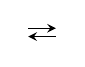
\begin{tikzpicture}[baseline]%
    \draw[>=stealth,<-](0,0.15ex)--(\arrlen,0.15ex);%
    \draw[>=stealth,->](0,0.85ex)--(\arrlen,0.85ex);%
  \end{tikzpicture}}}
\newcommand{\doubto}{\mathrel{%
  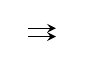
\begin{tikzpicture}[baseline]%
    \draw[>=stealth,->](0,0.15ex)--(\arrlen,0.15ex);%
    \draw[>=stealth,->](0,0.85ex)--(\arrlen,0.85ex);%
  \end{tikzpicture}}}
\newcommand{\lblto}[1]{\mathrel{%
    \begin{tikzpicture}[baseline= {( $ (current bounding box.south) + (0,-0.5ex) $ )}]
      \node[inner sep=.4ex] (a) {\,$\scriptstyle #1$\,};
      \draw[>=stealth,->] (a.south west) -- (a.south east);
    \end{tikzpicture}}}
\newcommand{\isoto}{\lblto{\sim}}

\newcommand{\simpl}[3]{
  \begin{tikzcd}[ampersand replacement=\&, column sep=small]
    #1 \&
    #2 \ar[l, shift right=0.35ex]
       \ar[l, shift left=0.35ex] \&
    #3 \ar[l, shift right=0.70ex]
       \ar[l, shift left=0.70ex]
       \ar[l] \&
    \cdots \ar[l, shift right=0.35ex]
           \ar[l, shift left=0.35ex]
           \ar[l, shift right=1.05ex]
           \ar[l, shift left=1.05ex]
  \end{tikzcd}
}
\newcommand{\cosimpl}[3]{
  \begin{tikzcd}[ampersand replacement=\&, column sep=small]
    #1 \ar[r, shift right=0.35ex]
       \ar[r, shift left=0.35ex] \&
    #2 \ar[r, shift right=0.70ex]
       \ar[r, shift left=0.70ex]
       \ar[r] \&
    #3 \ar[r, shift right=0.35ex]
       \ar[r, shift left=0.35ex]
       \ar[r, shift right=1.05ex]
       \ar[r, shift left=1.05ex] \&
    \cdots
  \end{tikzcd}
}

\newcommand{\tto}{\mathrel{\tikz[baseline]%
    \draw[>=stealth,->,double, double distance = 0.3ex](0,0.5ex)--(\arrlen,0.5ex);}}
\newcommand{\doubfrom}{\mathrel{%
  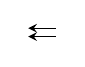
\begin{tikzpicture}[baseline]%
    \draw[>=stealth,<-](0,0.15ex)--(\arrlen,0.15ex);%
    \draw[>=stealth,<-](0,0.85ex)--(\arrlen,0.85ex);%
  \end{tikzpicture}}}
\newcommand{\tripfrom}{\mathrel{%
  
\begin{tikzpicture}[baseline]%
    \draw[>=stealth,<-](0,0.00ex)--(\arrlen,0.00ex);%
    \draw[>=stealth,<-](0,0.50ex)--(\arrlen,0.50ex);%
    \draw[>=stealth,<-](0,1.00ex)--(\arrlen,1.00ex);%
  \end{tikzpicture}}}


\renewcommand{\l}{\left}
\renewcommand{\r}{\right}
\newcommand{\f}{\frac}
\renewcommand{\o}{\overline}
\renewcommand{\u}{\underline}
\newcommand{\til}{\widetilde}
\renewcommand{\hat}{\widehat}
\newcommand{\del}{\partial}
\newcommand{\dash}{\text{-}}
\renewcommand{\c}{\colon}
\newcommand{\lc}{\,:\!}
\newcommand{\ce}{\coloneq}%{\mathrel{:=}}
\newcommand{\ec}{\eqcolon}%{\mathrel{=:}}
\newcommand{\iso}{\simeq}
\newcommand{\dual}{\vee}
\newcommand{\ldb}{\llbracket}
\newcommand{\rdb}{\rrbracket}

\newcommand{\Obj}{\operatorname{Obj}}
\newcommand{\Hom}{\operatorname{Hom}}
\newcommand{\Map}{\operatorname{Map}}
\newcommand{\Fun}{\operatorname{Fun}}
\newcommand{\Aut}{\operatorname{Aut}}
\newcommand{\Iso}{\operatorname{Iso}}
\renewcommand{\id}{\mathrm{id}}
\renewcommand{\im}{\operatorname{im}}
\newcommand{\op}{\mathrm{op}}
\newcommand{\univ}{\mathrm{univ}}
\newcommand{\colim}{\operatorname*{colim}}
\newcommand{\dlim}{\displaystyle\lim}
\newcommand{\dcolim}{\displaystyle\colim}
\newcommand{\Spec}{\operatorname{Spec}}
\newcommand{\Spf}{\operatorname{Spf}}

%%%%%%%%%%%%%%%%%%%%%%%%%%%%%%%%%%%%%%%%%%%%%%%%%%%%%%%%%%%%%%%%%%%%%%


\title{K\"ahler differentials}
\author{Arpon Raksit}
\date{January 27, 2016}

 \numberwithin{equation}{section}
% \cspreto{section}{\setcounter{equation}{0}}

\begin{document}
\maketitle

\newcommand{\Der}{\mathrm{Der}}
\newcommand{\Mod}{\mathrm{Mod}}
\newcommand{\Alg}{\mathrm{Alg}}
\newcommand{\Set}{\mathrm{Set}}
\renewcommand{\Top}{\mathrm{Top}}
\newcommand{\pre}{\mathrm{pre}}
\newcommand{\Op}{\mathrm{Op}}

%%%%%%%%%%%%%%%%%%%%%%%%%%%%%%%%%%%%%%%%%%%%%%%%%%%%%%%%%%%%%%%%%%%%%%

\section{Preliminaries}

\begin{convention}
  \label{rings-commutative}
  All rings and algebras are commutative and unital.
\end{convention}

\begin{notation}
  \label{open-poset}
  If $X$ is a topological space, we denote the (po)set of open subsets of $X$ by $\Op(X)$.
\end{notation}

\begin{notation}
  \label{locring-maps}
  Let $(X,\sO_X)$ and $(Y,\sO_Y)$ be ringed spaces. Recall that a map of ringed spaces $(X,\sO_X) \to (Y,\sO_Y)$ consists of a continuous map $\pi \c X \to Y$ together with a map $\alpha \c \pi^{-1}\sO_Y \to \sO_X$ of sheaves of rings on $X$ (or equivalently $\alpha \c \sO_Y \to \pi_*\sO_Y$ on $Y$). Thus we will denote maps of ringed spaces by pairs $(\pi,\alpha)$.
\end{notation}

\begin{definitions}
  \label{groth-cats}
  \begin{enumerate}[leftmargin=*]
  \item \label{mod-cat}
    Let $\Mod$ denote the category with:
    \begin{itemize}
    \item objects given by pairs $(A,M)$, where $A$ is a ring and $M$ is an $A$-module;
    \item morphisms $(A,M) \to (B,N)$ are given by triples $(\alpha,\phi)$ where $\alpha$ is a map of rings $A \to B$ and $\phi$ is a map of $A$-modules $M \to N$.
    \end{itemize}
  \item \label{topmod-cat}
    Let $\Top\Mod$ denote the category with:
    \begin{itemize}
    \item objects given by triples $(X,\sO_X,M)$, where $(X,\sO_X)$ is a ringed space and $M$ is an $\sO_X$-module;
    \item morphisms $(X,\sO_X,M) \to (Y,\sO_Y,N)$ are given by triples $(\pi,\alpha,\phi)$ where $(\pi,\alpha)$ is a map of ringed spaces $(X,\sO_X,M) \to (Y,\sO_Y,N)$ and $\phi$ is a map of $\sO_X$-modules $\pi^*N \to M$ (or equivalently a map of $\sO_Y$-modules $N \to \pi_*M$).
    \end{itemize}
    Observe that the full subcategory of $\Top\Mod$ on objects $(X,\sO_X,M)$ for which $X$ is a point is canonically equivalent to the category $\Mod^\op$.
  \item \label{alg-cat}
    Let $\Alg$ denote the arrow category of rings, i.e. the category with:
    \begin{itemize}
    \item objects given by maps of rings $A \to B$;
    \item morphisms from $A \to B$ to $A' \to B'$ given by commutative squares
      \[
        \begin{tikzcd}
          B \ar[r] & B' \\
          A \ar[r] \ar[u] & A' \ar[u].
        \end{tikzcd}
      \]
    \end{itemize}
  \item \label{topalg-cat}
    Let $\Top\Alg$ denote the arrow category of ringed spaces, i.e. the category with:
    \begin{itemize}
    \item objects given by maps of ringed spaces $(X,\sO_X) \to (Y,\sO_Y)$;
    \item morphisms from $(X,\sO_X) \to (Y',\sO_Y')$ to $(X,\sO_{X'}) \to (Y',\sO_{Y'})$ given by commutative squares
      \[
      \begin{tikzcd}
        (X,\sO_X) \ar[r] \ar[d] & (X',\sO_{X'}) \ar[d] \\
        (Y,\sO_Y) \ar[r] & (Y',\sO_{Y'}).
      \end{tikzcd}
      \]
    \end{itemize}
    Observe that the full subcategory of $\Top\Alg$ on objects $(X,\sO_X) \to (Y,\sO_Y)$ for which $X$ and $Y$ are points is canonically equivalent to the category $\Alg^\op$.
  \end{enumerate}
\end{definitions}

%%%%%%%%%%%%%%%%%%%%%%%%%%%%%%%%%%%%%%%%%%%%%%%%%%%%%%%%%%%%%%%%%%%%%%

\section{Derivations and differentials}

In this section we fix a map of ringed spaces $(\pi,\alpha) \c (X,\sO_X) \to (Y,\sO_Y)$.

\begin{definition}
  \label{derivation}
  Let $M$ be an $\sO_X$-module. A \emph{$Y$-derivation on $X$ in $M$} is
  a map of $\pi^{-1}\sO_Y$-modules $d \c \sO_X \to M$ satisfying the Leibniz rule,
  \[
    d(fg) = f\,d(g) + d(f)\,g \quad
    \text{for}\ f,g \in \sO_X(U),\ U \in \Op(X).
  \]
\end{definition}

\begin{remark}
  \label{derivation-kills-constants}
  Note that the Leibniz rule implies
  \[
    d(1) = d(1 \cdot 1) = 1 \cdot d(1) + d(1) \cdot 1 = 2 \cdot d(1)
    \implies d(1) = 0;
  \]
  and by $\pi^{-1}\sO_Y$-linearity this implies more generally that
  $d \circ \alpha = 0$. Conversely, if $d \c \sO_X \to M$ is a map of
  sheaves of abelian groups satisfying the Leibniz rule, then the
  condition $d \circ \alpha = 0$ clearly implies that $d$ is
  $\pi^{-1}\sO_Y$-linear.
\end{remark}

\begin{notation}
  \label{derivation-functor}
  Denote the set of $Y$-derivations on $X$ in $M$ by $\Der(X/Y,M)$. If $d \c \sO_X \to M$ is a $Y$-derivation and $\phi \c M \to N$ a map of $\sO_X$-modules, then $\phi \circ d \c \sO_X \to N$ is a $Y$-derivation on $X$ in $N$. Thus the assignment $M \mapsto \Der(X/Y,M)$ defines a functor $\Mod_{\sO_X} \to \Set$.
\end{notation}

\begin{definition}
  \label{kahler-def}
  We define the $\sO_X$-module $\Omega_{X/Y}$ of \emph{K\"ahler differentials on $X$ over $Y$} to be an object corepresenting the functor $\Der(X/Y,-) \c \Mod_{\sO_X} \to \Set$. That is, $\Omega_{X,Y}$ is defined by the property that there is a \emph{universal $Y$-derivation} $d$ on $X$ in $\Omega_{Y/X}$, where ``universal'' means as usual that composition with $d$ gives an isomorphism
  \[
    \Hom_{\Mod_{\sO_X}}(\Omega_{X/Y}, M) \iso \Der(X/Y,M).
  \]
  Of course, this property uniquely characterizes $\Omega_{X/Y}$, but it remains to prove its existence. We do so in \cref{kahler-constr}.
\end{definition}

\begin{remark}
  \label{kahler-functor}
  This definition \cref{kahler-def} takes in as input a map $(\pi,\alpha) \c (X,\sO_X) \to (Y,\sO_Y)$, i.e. an object of $\Top\Alg$, and outputs an $\sO_X$-module $\Omega_{X/Y}$, i.e. an object $(X, \sO_X, \Omega_{X/Y}) \in \Top\Mod$.

  Suppose
  \[
    \begin{tikzcd}
      (X,\sO_X) \ar[r, "{(\sigma,\gamma)}"] \ar[d, "{(\pi,\alpha)}", swap] &
      (X',\sO_{X'}) \ar[d, "{(\rho,\beta)}"] \\
      (Y,\sO_Y) \ar[r, "{(\tau,\delta)}"] &
      (Y',\sO_{Y'})
    \end{tikzcd}
  \]
  is a commutative diagram, i.e. a map in $\Top\Alg$. Let $M$ be an $\sO_X$-module. There is a map of sets $\Der(X/Y,M) \to \Der(X'/Y',\sigma_*M)$ defined as follows: given a $Y$-derivation $\sO_X \to M$, restrict in $\gamma$ to obtain a map $\sigma^{-1}\sO_{X'} \to M$, then pass to the adjoint map $\sigma \c \sO_{X'} \to \sigma_*M$, which one easily checks is a $Y'$-derivation.

  This is clearly natural in $M$, so we have defined a natural transformation $\Der(X/Y,-) \to \Der(X'/Y',\sigma_*(-))$. By definition of K\"ahler differentials \cref{kahler-def}, this is equivalent to a natural transformation
  \[
    \Hom_{\Mod_{\sO_X}}(\Omega_{X/Y},-) \to
    \Hom_{\Mod_{\sO_{X'}}}(\Omega_{X'/Y'},\sigma_*(-)) \iso
    \Hom_{\Mod_{\sO_X}}(\sigma^*\Omega_{X'/Y'},-),
  \]
  which, by the Yoneda lemma, is equivalent to a map of $\sO_X$-modules $\phi \c \sigma^*\Omega_{X'/Y'} \to \Omega_{X/Y}$, determining a map $(\sigma,\gamma,\phi) \c (X, \sO_X, \Omega_{X/Y}) \to (X', \sO_{X'}, \Omega_{X'/Y'})$ in $\Top\Mod$. Thus, the assignment of K\"ahler differentials
  \[
    (\pi,\alpha) \c (X,\sO_X) \to (Y,\sO_Y)
    \quad \mapsto \quad
    (X, \sO_X, \Omega_{X/Y})
  \]
  defines a functor $\Omega \c \Top\Alg \to \Top\Mod$.
\end{remark}

\begin{remark}
  \label{kahler-restricted}
  Note that when restricted to the full subcategory $\Alg^\op \inj \Top\Alg$ \cref{topalg-cat}, the K\"ahler differentials functor $\Omega$ defined in \cref{kahler-functor} takes values in the full subcategory $\Mod^\op \inj \Top\Mod$ \cref{topmod-cat}. I.e. $\Omega$ restricts to a functor $\Alg \to \Mod$, given by the assignment $(A \to B) \mapsto (B, \Omega_{B/A})$.

  In general, when we restrict to $\Alg$, i.e. when $X$ and $Y$ are points, we replace $X$ and $Y$ in our terminology and notation with $B$ and $A$. E.g. we have \emph{$A$-derivations on $B$} in $B$-modules $M$, the set of such derivations is denoted $\Der(B/A,M)$, and as above, the $B$-module of \emph{K\"ahler differentials of $B$ over $A$} is denoted $\Omega_{B/A}$.
\end{remark}

\begin{construction}
  \label{kahler-constr}
  We now construct the object $\Omega_{X/Y}$ defined in \cref{kahler-def}, proving its existence. We start by doing this for the case that $X$ and $Y$ are points. Our notation is as discussed in \cref{kahler-restricted}: we consider a ring map $\alpha \c A \to B$ and construct $\Omega_{B/A}$. This is straightforward: we define $\Omega_{B/A}$ to be the $B$-module generated by symbols $\{df\}_{f \in B}$, subject only to the required relations:
  \[
    d(f+g) = df + dg, \qquad
    d(fg) = f(dg) + (df)g, \qquad
    d\alpha(c) = 0,
  \]
  for $f,g \in B$ and $c \in A$. Then the universal $A$-derivation $d \c B \to \Omega_{B/A}$ is given simply by $f \mapsto df$.

  We now return to the general case. Applying the previous construction locally, we obtain a pre-$\sO_X$-module $\Omega_{X/Y}^\pre$ by assigning to $U \in \Op(X)$ the K\"ahler differentials of $\sO_X(U)$ over $\pi^{-1}\sO_Y(U)$; i.e. we define
  \[
    \Omega_{X/Y}^\pre(U) \ce \Omega_{\sO_X(U)/\pi^{-1}\sO_Y(U)} \in \Mod_{\sO_X(U)}.
  \]
  Finally, we define $\Omega_{X/Y} \in \Mod_{\sO_X}$ to be the sheafification of $\Omega_{X/Y}^\pre$.
\end{construction}

%%%%%%%%%%%%%%%%%%%%%%%%%%%%%%%%%%%%%%%%%%%%%%%%%%%%%%%%%%%%%%%%%%%%%%

\section{Square-zero extensions}

\begin{construction}
  \label{square-zero}
  Let $(X,\sO_X)$ be a ringed space and $M$ an $\sO_X$-module. We construct an $\sO_X$-algebra $A \oplus M$, called the \emph{square-zero extension of $\sO_X$ by $M$}. As the notation suggests, the underlying $\sO_X$-module is the direct sum $\sO_X \oplus M$. And as the name suggests, the ring structure is defined by requiring:
  \begin{itemize}
  \item that $M$ (or rather its image in the canonical inclusion $M \to \sO_X \oplus M$) be a square-zero ideal in $\sO_X \oplus M$;
  \item that the canonical inclusion $\iota_{X,M} \c \sO_X \to \sO_X \oplus M$ be a ring map (so that we indeed get an $\sO_X$-algebra).
  \end{itemize}
  These conditions lead to the following formula for multiplication:
  \[
    (f,m)(g, n) = (fg, fn + gm) \quad \text{for}\ (f,m), (g,n) \in (\sO_X \oplus M)(U),\ U \in \Op(X),
  \]
  noting that $(\sO_X \oplus M)(U) \iso \sO_X(U) \oplus M(U)$.
\end{construction}

\begin{remark}
  \label{square-zero-functor}
  This construction \cref{square-zero} takes in as input a triple $(X,\sO_X,M) \in \Top\Mod$ and outputs an $\sO_X$-algebra $\iota_{X,M} \c \sO_X \to \sO_X \oplus M$, which we may interpret as an object $(\id_X,\iota_{X,M}) \c (X,\sO_X \oplus M) \to (X, \sO_X)$ in $\Top\Alg$.

  Moreover, if $(\pi,\alpha,\phi)$ is a map $(X,\sO_X,M) \to (Y,\sO_Y,N)$ in $\Top\Mod$, then the diagram
  \[
    \begin{tikzcd}[column sep = large]
      (X,\sO_X \oplus M)
        \ar[r, "{(\pi, \alpha \oplus \phi)}"] \ar[d, "{(\id_X,\iota_{X,M})}" ] &
      (Y,\sO_Y \oplus N) \ar[d, "{(\id_Y,\iota_{Y,N})}"] \\
      (X,\sO_X) \ar[r, "{(\pi,\alpha)}"] &
      (Y,\sO_Y)
    \end{tikzcd}
  \]
  is a map $(\id_X,\iota_{X,M}) \to (\id_Y,\iota_{Y,N})$ in $\Top\Alg$. Thus the square-zero extension construction
  \[
    (X, \sO_X, M)
    \quad \mapsto \quad
    (\id_X, \iota_{X,M}) \c (X, \sO_X \oplus M) \to (X, \sO_X)
  \]
  defines a functor $\oplus \c \Top\Mod \to \Top\Alg$.
\end{remark}

\begin{remark}
  \label{square-zero-restricted}
  Note that when restricted to the full subcategory $\Mod^\op \inj \Top\Mod$ \cref{topmod-cat}, the square-zero extension functor $\oplus$ defined in \cref{square-zero-functor} takes values in the full subcategory $\Alg^\op \inj \Top\Alg$ \cref{topalg-cat}. I.e. $\oplus$ restricts to a functor $\Mod \to \Alg$, given by the assignment $(A,M) \mapsto (A \to A \oplus M)$.
\end{remark}

\begin{lemma}
  \label{derivation-square-zero}
  Let $(Z,\sO_Z)$ be a ringed space and $M$ an $\sO_Z$-module. Let $(\pi,\alpha) \c (X,\sO_X) \to (Y,\sO_Y)$ be a map of ringed spaces. Then the following data are equivalent:
  \begin{itemize}
  \item a map from $(\id_Z,\iota_{Z,M}) \c (Z, \sO_Z \oplus M) \to (Z, \sO_Z)$ to $(\pi,\alpha) \c (X,\sO_X) \to (Y,\sO_Y)$ in $\Top\Alg$;
  \item a map of ringed spaces $(\rho,\beta) \c (Z,\sO_Z) \to (X,\sO_X)$ together with a $Y$-derivation on $X$ in $\rho_*M$.
  \end{itemize}
  Moreover, the bijection between the sets of these data is functorial in $(Z,\sO_Z,M) \in \Mod^\op$ and $(\pi,\alpha) \in \Top\Alg$.
\end{lemma}

\begin{proof}
  This boils down to the following fact, which is straightforwardly verified. Let $\gamma \c \sO_X \to \rho_*\sO_Z \oplus \rho_*M$ be a map of sheaves of sets. Write $\gamma = (\beta,d)$ for maps $\beta \c \sO_X \to \rho_*\sO_Z$ and
  $d \c \sO_X \to \rho_*M$. Then the following are equivalent:
  \begin{itemize}
  \item $\gamma$ is a map of sheaves of rings whose restriction $\gamma \circ \alpha \c \pi^{-1}\sO_Y \to \rho_*\sO_Z \oplus \rho_*M$ factors through $\rho_*\sO_Z$.
  \item $\beta$ is a map of sheaves of rings and $d$ is a $Y$-derivation. \qedhere
  \end{itemize}
\end{proof}

\begin{proposition}
  \label{kahler-adjunction}
  There is an adjunction
  \[
    \oplus \c \Top\Mod \fromto \Top\Alg \lc \Omega,
  \]
  where the left adjoint $\oplus$ denotes the square-zero extension functor \cref{square-zero-functor}, and the right adjoint $\Omega$ denotes the K\"ahler differentials functor \cref{kahler-functor}.
\end{proposition}

\begin{proof}
  Combine \cref{derivation-square-zero} with the definition of K\"ahler differentials \cref{kahler-def}.
\end{proof}

\begin{corollary}
  \label{kahler-adjunction-restricted}
  By restricting the adjunction supplied by \cref{kahler-adjunction} to the full subcategories $\Mod^\op \inj \Top\Mod$ and $\Alg^\op \inj \Top\Mod$ \cref{kahler-restricted,square-zero-restricted}, we obtain an adjunction
  \[
    \Omega \c \Alg \fromto \Mod \lc \oplus,
  \]
  where now (after taking opposite categories) K\"ahler differentials $\Omega$ is left adjoint to square-zero extension $\oplus$.
\end{corollary}

%%%%%%%%%%%%%%%%%%%%%%%%%%%%%%%%%%%%%%%%%%%%%%%%%%%%%%%%%%%%%%%%%%%%%%

\section{Properties of differentials}

\begin{lemma}
  \label{differentials-stalk}
  Let $(\pi,\alpha) \c (X,\sO_X) \to (Y,\sO_Y)$ be a map of ringed spaces. Let $x \in X$. Then the stalk of the K\"ahler differentials sheaf $\Omega_{X/Y}$ at $x$ is given by the K\"ahler differentials module of the ring map of stalks $\alpha_x \c \sO_{Y,\pi(x)} \to \sO_{X,x}$. That is, there is a canonical isomorphism of $\sO_{X,x}$-modules $(\Omega_{X/Y})_x \iso \Omega_{\sO_{X,x}/\sO_{Y,\pi(x)}}$.
\end{lemma}

\begin{proof}
  Recall from \cref{kahler-constr} that $\Omega_{X/Y}$ is the sheafification of the presheaf $\Omega_{X/Y}^\pre$ defined by the assignment
  \[
    \Op(X) \ni U \mapsto \Omega_{\sO_X(U)/\pi^{-1}\sO_Y(U)} \in \Mod_{\sO_X(U)}.
  \]
  Since sheafification preserves stalks, it follows that
  \[
    (\Omega_{X/Y})_x
    \iso (\Omega_{X/Y}^\pre)_x
    \iso \colim_{U \ni x} \Omega_{X/Y}^\pre(U)
    \iso \colim_{U \ni x} \Omega_{\sO_X(U)/\pi^{-1}\sO_Y(U)}.
  \]
  As this is a filtered colimit (taken over the poset of $U \in \Op(X)$ containg $x$), it also computes the colimit inside the category $\Mod$; more precisely, we have isomorphisms
  \begin{align*}
    (\sO_{X,x}, (\Omega_{X/Y})_x) &\iso
    \colim_{U \ni x} {(\sO_X(U), \Omega_{\sO_X(U)/\pi^{-1}\sO_Y(U)})} \\ &\iso
    \colim_{U \ni x} \Omega(\alpha_U \c \pi^{-1}\sO_Y(U) \to \sO_X(U))
  \end{align*}
  in $\Mod$. By \cref{kahler-adjunction-restricted}, $\Omega \c \Alg \to \Mod$ is a left adjoint and hence preserves colimits, so we obtain an isomorphism (still in $\Mod$)
  \[
    (\sO_{X,x}, (\Omega_{X/Y})_x) \iso
    \Omega\l(\colim_{U \ni x} \alpha_U\r) \iso
    \Omega(\alpha_x),
  \]
  which is the desired isomorphism of $\sO_{X,x}$-modules $(\Omega_{X/Y})_x \iso \Omega_{\sO_{X,x}/\sO_{Y,\pi(x)}}$.
\end{proof}

\begin{lemma}
  Let $k$ be a field and $A$ a $k$-algebra. Suppose $A$ is a local ring with maximal ideal $\km$ and residue field $k$, i.e. such that the map $k \to A/\km$ is an isomorphism. Then there is an isomorphism of $k$-vector spaces $\Omega_{A/k} \otimes_A k \iso \km/\km^2$.
\end{lemma}



%%%%%%%%%%%%%%%%%%%%%%%%%%%%%%%%%%%%%%%%%%%%%%%%%%%%%%%%%%%%%%%%%%%%%%

% \bibliographystyle{amsalpha}
% \bibliography{refs}

\end{document}
